\documentclass{article}

\usepackage[utf8x]{inputenc}
\usepackage[english,russian]{babel}
\usepackage{cmap}
\usepackage{commath}
\usepackage{amsmath}
\usepackage{amsfonts}
\usepackage{mathtools}
\usepackage{amssymb}
\usepackage{parskip}
\usepackage{titling}
\usepackage{color}
\usepackage{hyperref}
\usepackage{cancel}
\usepackage{enumerate}
\usepackage{multicol}
\usepackage{graphicx}
\usepackage[font=small,labelfont=bf]{caption}
\usepackage[a4paper, left=2.5cm, right=1.5cm, top=2.5cm, bottom=2.5cm]{geometry}

\graphicspath{ {./images/} }
\setlength{\droptitle}{-3cm}
\hypersetup{ colorlinks=true, linktoc=all, linkcolor=blue }
\pagenumbering{arabic}

\begin{document}
    \subsection{Первый замечательный предел}
    \( \lim_{x \rightarrow 0} \frac{sin\ x}{x} = 1;\ \lim_{x \rightarrow 0+} f(x) = \lim_{x \rightarrow 0-} f(x) \rightarrow\ \exists \lim_{x \rightarrow 0} f(x) = A \)
    
    \begin{enumerate}
        \item Пусть \(0 < x < \frac{\pi}{2}\)
        
        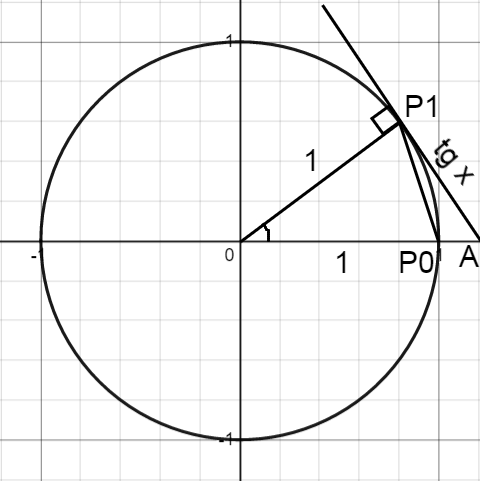
\includegraphics[scale=0.35]{11_1_4_1.png}

        \( S_{OP_1P_0} < S_{\textrm{сект}} < S_{OP_1A}  \)
        
        \(\not \frac{1}{2} \cdot 1 \cdot 1 \cdot sin\ x < \not \frac{1}{2} x < \not \frac{1}{2} \cdot 1 \cdot tg\ x \Rightarrow\)
        
        \(\Rightarrow \frac{1}{tg\ x} < \frac{1}{x} < \frac{1}{sin\ x}\)\\
        \(cos\ x < \frac{sin\ x}{x} < 1\)

        \(cos\ x \xrightarrow[]{x \rightarrow 0+} 1\)\\
        \(1 \xrightarrow[]{x \rightarrow 0+} 1\)

        \(\xRightarrow[]{\textrm{по теореме о 2х милиционерах}} lim_{x \rightarrow 0+} \frac{sin\ x}{x} = 1\)

        \item \( \lim_{x \rightarrow 0-} \frac{sin\ x}{x} = 
        \begin{cases}
            t = -x\\
            t \rightarrow 0+    
        \end{cases} = lim_{t \rightarrow 0+} \frac{sin(-t)}{-t} = lim_{t \rightarrow 0+} \frac{-sin(t)}{-t} = 1
        \)
        \item \( lim_{x \rightarrow 0+} \frac{sin(x)}{x} = lim_{x \rightarrow 0-} \frac{sin(x)}{x} = 1 \Rightarrow lim_{x \rightarrow 0} \frac{sin(x)}{x} = 1 \)
    \end{enumerate}
    \textbf{Примеры.}

    \begin{enumerate}
        \item \( lim_{x \rightarrow 0} \frac{tg(x)}{x} = lim_{x \rightarrow 0} \frac{sin(x)}{x}\frac{1}{cos(x)} = 1 \)
        \item \( lim_{x \rightarrow 0} \frac{(sin(5x)) 5x}{(5x) 8x} = lim_{x \rightarrow 0} \frac{sin(5x)}{5x} \cdot lim_{x \rightarrow 0} \frac{5}{8} = \frac{5}{8}\)
    \end{enumerate}
    
    \( lim_{x \rightarrow +\infty} \frac{sin(x)}{x} = 0\)\\
    Не путать с первым замечательным пределом

    \subsection{Точная верхняя и точная нижняя грани множества}
    \( \mathbb{E} \) --- числовое множество\\
    \( \mathbb{Z} \) --- неограничено\\
    \( \mathbb{N} \) --- неограничено сверху, снизу ограничено \( min = 1 \)\\
    \( [a; b] \) --- ограничено снизу, ограничено сверху \( min = a, max = b \)\\
    \( (0; 1] \) --- ограничено \( max +;  min - \); 0 --- точная верхняя грань, 1 --- точная нижняя грань

    \textbf{Определение.} Конечное число \(M\) называется точной верхней гранью множества \(\mathbb{E}\)\\ 
    \(M = sup\ \mathbb{E} - "supremum")\), если
    \begin{enumerate}
        \item \( \forall x \in \mathbb{E}\ x \leq M \)
        \item \( \forall \varepsilon > 0\ \exists x_1 \in \mathbb{E}:\ M - \varepsilon < x_1 \leq M \)
    \end{enumerate}
    
    \textbf{Определение.} Конечное число \(m\) называется точной нижней гранью множества \(\mathbb{E}\)\\
    \(m = inf\ \mathbb{E} - "infimum")\), если
    \begin{enumerate}
        \item \( \forall x \in \mathbb{E}\ m \leq x \)
        \item \( \forall \varepsilon > 0\ \exists x_1 \in \mathbb{E}:\ m \leq x_1 < m + \varepsilon \)
    \end{enumerate}

    \textbf{Пример.}
    
    \( \mathbb{E} = \{ \frac{n}{n + 1}, n \in \mathbb{N} \} = \{ \frac{1}{2}; \frac{2}{3}; \frac{3}{4}; ... \} \)\\
    \( inf\ \mathbb{E} = \frac{1}{2} = min \mathbb{E} \)

    \(max\ \mathbb{E} = \emptyset\)\\
    \(sup\ \mathbb{E} = 1\) --- ?

    \(\uparrow\)
    \begin{enumerate}
        \item \(\forall x \in \mathbb{E}\ \frac{n}{n+1} \leq^{?} 1\ \frac{n}{n+1} = 1 - \frac{1}{n+1} < 1\)
        \item \( \forall \varepsilon > 0\ \exists x_1 = \frac{n_1}{n_1 + 1} \)
        
        \( 1 - \varepsilon < \frac{n_1}{n_1 + 1} \leq 1 \)

        \( 1 - \varepsilon < 1 - \frac{1}{n_1 + 1} \)
        
        \( 0 < \frac{1}{n_1 + 1} < \varepsilon_{> 0} \)

        \( \frac{1}{\varepsilon} < n_1 + 1 \)

        \( n_1 > \frac{1}{\varepsilon} - 1\)
        
        ч.т.д.
    \end{enumerate}
    \(\downarrow\)
    
    \textbf{Теорема.} Если числовое множество \(\mathbb{E}\) ограничено сверху(снизу), то для него существует \(sup\ \mathbb{E}(inf\ \mathbb{E})\).

    Если числовое множество \(\mathbb{E}\)  
    \begin{enumerate}
        \item неограничено сверху, то \(sup\ \mathbb{E} \stackrel{df}{=} +\infty\)
        \item неограничено снизу, то \(inf\ \mathbb{E} \stackrel{df}{=} -\infty\)
    \end{enumerate}

    \subsection{Функции, непрерывные на отрезке}
    \textbf{Определение.} Функция \( y = f(x) \) называется непрерывной на отрезке \( [a, b] \), если она непрерывна в любой \( x \in (a, b) \); непрерывна в \( x = a \) справа и в \( x = b \) слева.


    \subsubsection{Теорема Коши}
    \textbf{Теорема.} Функция \( y = f(x) \) непрерывная на \( [a, b] \) ограничена на нем.

    \(\uparrow\) от противного

    \(\underline{\textrm{Неограничена на отрезке}}\), т.е.

    \(\forall n \in \mathbb{N}\ \exists x_n \in [a,b]:\ f(x_n)^{=y_n} > n\), но это означает, что \(lim_{n \rightarrow \infty} f(x_n) = +\infty\) (*),\\
    \underline{\underline{но}} \(x_n \in [a,b]\), т.е. \(\{x_n\}\) --- ограничена из ограниченной последовательности всегда можем выделить сходящуюся подпоследовательность\\
    \(\exists x_{nk}:\ x_{nk} \xrightarrow[k \rightarrow \infty]{} d \in [a,b]\)

    \(lim_{k \rightarrow \infty} f(x_{nk}) = f(d)\), это противоречит (*) \(\downarrow\)

    \textbf{Замечание.}
    \( y = \begin{cases}
        \frac{1}{x},\ x \neq 0\\
        0,\ x = 0
    \end{cases} \) на \( (0; 1] \)
    

    \subsubsection{Теорема Вейерштрасса}
    \textbf{Теорема.} Функция \( y = f(x) \) непрерывна на \( [a, b] \), то она достигает своего наибольшего и наименьшего значения. То есть \( \exists \alpha, \beta \in [a, b] \), такие что \( f(\alpha) = min_{x \in [a, b]} f(x)\); \( f(\beta) = max_{x \in [a, b]} f(x)\)
    \( f(\alpha) = min\ f(x); f(\beta) = max \)

    \(\uparrow\) по Т. Коши функция \(f(x)\) ограничена на \([a,b] \Rightarrow\ \exists inf\ f(x)\) и \(sup\ f(x) = M\)
    
    Докажем, что \(\exists max\), т.е. из \(\exists\)-ния \(sup\) 

    \begin{enumerate}
        \item \(f(x) \leq M\)
        \item \(\forall \varepsilon > 0\ \exists x_1 \in [a,b]:\ M - \varepsilon < f(x_1) \leq M\)
        Возьмём \(\varepsilon = \frac{1}{n} \Rightarrow\ \exists x_n:\\\)
        \(M - \frac{1}{n} < f(x_n) \leq M\\ \Rightarrow lim_{n \rightarrow \infty} f(x_n) = M\)

        \(x_n \in [a,b] \Rightarrow \{x_n\}\) --- ограничена \(\Rightarrow\ \exists\) подпоследовательность \(x_{nk}:\ x_{nk} \xrightarrow[k \rightarrow \infty]{} B \in [a, b]\).

        В силу непрерывности \( f(x) \) на \( [a, b]:\ lim_{k \to \infty} f(x_{nk}) = f(\beta) \).

        В силу единственности \( lim:\ f(\beta) = M \) --- это \( max \). \( \downarrow \)
    \end{enumerate}

    \textbf{Замечание.} 

    \( y = x \) на \( [0, 1) \) \( max \) значение не достигается\\
    \( sup_{[0, 1)} x = 1 \)


    \subsubsection{Теорема Больцано}
    \textbf{Теорема.} Если непрерывная на \([a, b]\) функция \(y = f(x):\ f(a) \cdot f(b) < 0\), то существует хотя бы одна \(c \in (a, b):\ f(c) = 0\).

    \( \uparrow \) пусть \( \sigma_0 = [a, b] \)

    \begin{enumerate}
        \item делим \( \frac{\sigma_0}{2} \); \( f(\frac{a + b}{2})\ ?\ 0 \)
        
        \( \sigma_1 = [a, \frac{a + b}{2}] \) или \( [\frac{a + b}{2}; b] \), чтобы на концах функция принимала значения разных знаков:\\
        если \(f(a) \cdot f(\frac{a+b}{2}) < 0\); если \(f(\frac{a+b}{2}) \cdot f(b) < 0\).
        
        \item \( \frac{\sigma_1}{2} \rightarrow \) если \(f(c_1) = 0\), то процесс завершился, иначе \(\sigma_2:\) на концах \(f\) принимает значение разных знаков \( \abs{\sigma_2} = \frac{b - 2}{2^2} \) и т.д. 
        
        Или 1) наткнемся на \( c: f(c) = 0 \)
        
        Или 2) \( \sigma_0 > \sigma_1 > \sigma_2 > ... \)
    \end{enumerate}
    
    \textbf{Замечание.}

    \(\abs{\sigma_n} = \frac{b-a}{2^n} \xrightarrow[n \rightarrow \infty]{} 0 \Rightarrow\ \exists !\) общая точка \(c\) этих вложенных промежутков. Очевидно, что \(f(c) = 0\)(если \(f(c) > 0\), то по т. о сохранении знака \(\exists U(c)\) в \(U(c) f(x) > 0\), но при больших \(n\ \exists \sigma_n \subset U(c);\) противоречие).

    \textbf{Следствие 1.} Если непрерывная на \([a, b]\) функция принимает значения \([m, M]\); где \(m = min\ f(x)(x \in [a, b]);\ M = max\ f(x)\) и \(c \in (m, M)\), то \(\exists x_0 \in [a,b]:\ f(x_0) = c\).
    
    \( \uparrow \) Если \( c = m \), то по т. Вейерштрасса \( \exists \alpha \). \( c = M \), то по т. Вейерштрасса \( \exists \beta \).

    \( c \in (m; M) \), то рассмотрим вспомогательную функцию \( f_1(x) = f(x) - c \). \( f_1(x) \) непрерывна на \( [a; b] \).\\
    \( f_1(\alpha) = f(\alpha) - c = m - c < 0 \)\\
    \( f_1(\beta) = M - c > 0 \)

    Т.е. \(f_1(x)\) непрерывна на отрезке \( [\alpha; \beta] \) (или \( [\beta; \alpha] \)) и \( f_1(\alpha) \cdot f_1(\beta) < 0 \Rightarrow \) по т. Больцано \( \exists x_0 \in [\alpha; \beta]([\beta; \alpha]): f_1(x_0) = 0 = f(x_0) - k \Rightarrow f(x_0) = k \downarrow \)

    \textbf{Следствие 2.} Если \( f(x) \) --- непрерывна на \( [a, b] \) и \( f(a) = f(b) = 0 \), и \(\nexists\) на \( [a, b] \) других точек, в которых \( f(x) \) обращается в ноль, то \( f(x) \) сохраняет знак \( (>0; <0) \) на всем \( (a, b) \).

    \(\uparrow\) От противного.

    Пусть на \((a; b)\ \exists x'; x'' :\ f(x')f(x'') < 0\), но тогда по т. Больцано на отрезке с концами \(x', x''\ \exists c:\ f(c)=0\), противоречие. \(\downarrow\)

    \textbf{Примеры:}

    \begin{enumerate}
        \item \(cos\ x - x = 0\) имеет хотя бы 1 решение на \((0; \pi)\)

        \(f(x) = cos\ x - x\) непрерывна на \([0; \pi]\).
    
        \(f(0) = cos\ 0 - 0 = 1 > 0\)\\
        \(f(\pi) = cos\ \pi - \pi = -1-\pi < 0\), по т. Больцано \(\exists c \in (0; \pi);\ f(c)=0\)

        \item \( \frac{x(x - 2)}{x + 3} > 0 \)

        (Решается методом интервалов)
    \end{enumerate}
    
\end{document}
